\documentclass[10pt,a4paper]{article}
\usepackage[latin1]{inputenc}
\usepackage{amsmath}
\usepackage{amsfonts}
\usepackage{amssymb}
\usepackage{graphicx}
\usepackage{hyperref} 
\usepackage{multirow}
\usepackage{makecell}
\usepackage{enumitem}
\usepackage{amsbsy,latexsym,tabulary,times,xcolor}
\usepackage{booktabs}
\usepackage{arydshln}
%\usepackage[nonindentfirst]{titlesec}
\usepackage{caption,abstract,fancyhdr}
%\usepackage[utf8]{inputenc}
%\usepackage[numbers,sort&compress]{natbib}
%\def\oupIndent{1pt}

\usepackage[T1]{fontenc}
%\usepackage[paperheight=297mm,paperwidth=210mm,columnsep=1.93pc,right=17.5mm,left=20mm,top=20mm,bottom=20mm]{geometry}
%\usepackage[margin=1.5cm,columnsep=1.93pc,top=1in,bottom=2cm]{geometry}
\usepackage[paperheight=11.69in,paperwidth=8.27in,margin=1.5cm,headsep=.5cm,top=2cm,bottom=2.5cm,columnsep=12pt]{geometry}
\linespread{1.2} \date{}
\captionsetup[table]{labelfont={bf},labelsep=period}
\captionsetup[figure]{labelfont={bf},labelsep=period}
\def\abstractname{\fontsize{16pt}{19.2pt}\sffamily{Abstract}\selectfont}
\renewenvironment{onecolabstract} {\vspace*{-1pc}\trivlist\item[]\leftskip\oupIndent\par\vskip4pt\noindent\textit{{\abstractname}}\mbox{\null}\\ \textcolor[cmyk]{.77,.49,.38,.11}{\rule[.5pc]{\textwidth}{2pt}} \newline}{\par\noindent\endtrivlist}

%\renewcommand{\bibnumfmt}[1]{#1.}

\usepackage{colortbl}
\usepackage{xcolor}
\usepackage{pifont}
\usepackage[nointegrals]{wasysym}
\urlstyle{rm}

\usepackage[colorinlistoftodos,textsize=scriptsize]{todonotes}

\begin{document}
	
\newcolumntype{H}{>{\setbox0=\hbox\bgroup}c<{\egroup}@{}}

\section*{Appendix} 
\label{chp:appendix}

% Reason to have set U <= 40 for experiments with CLEF 2016

\begin{figure}[h!]
	\centering
	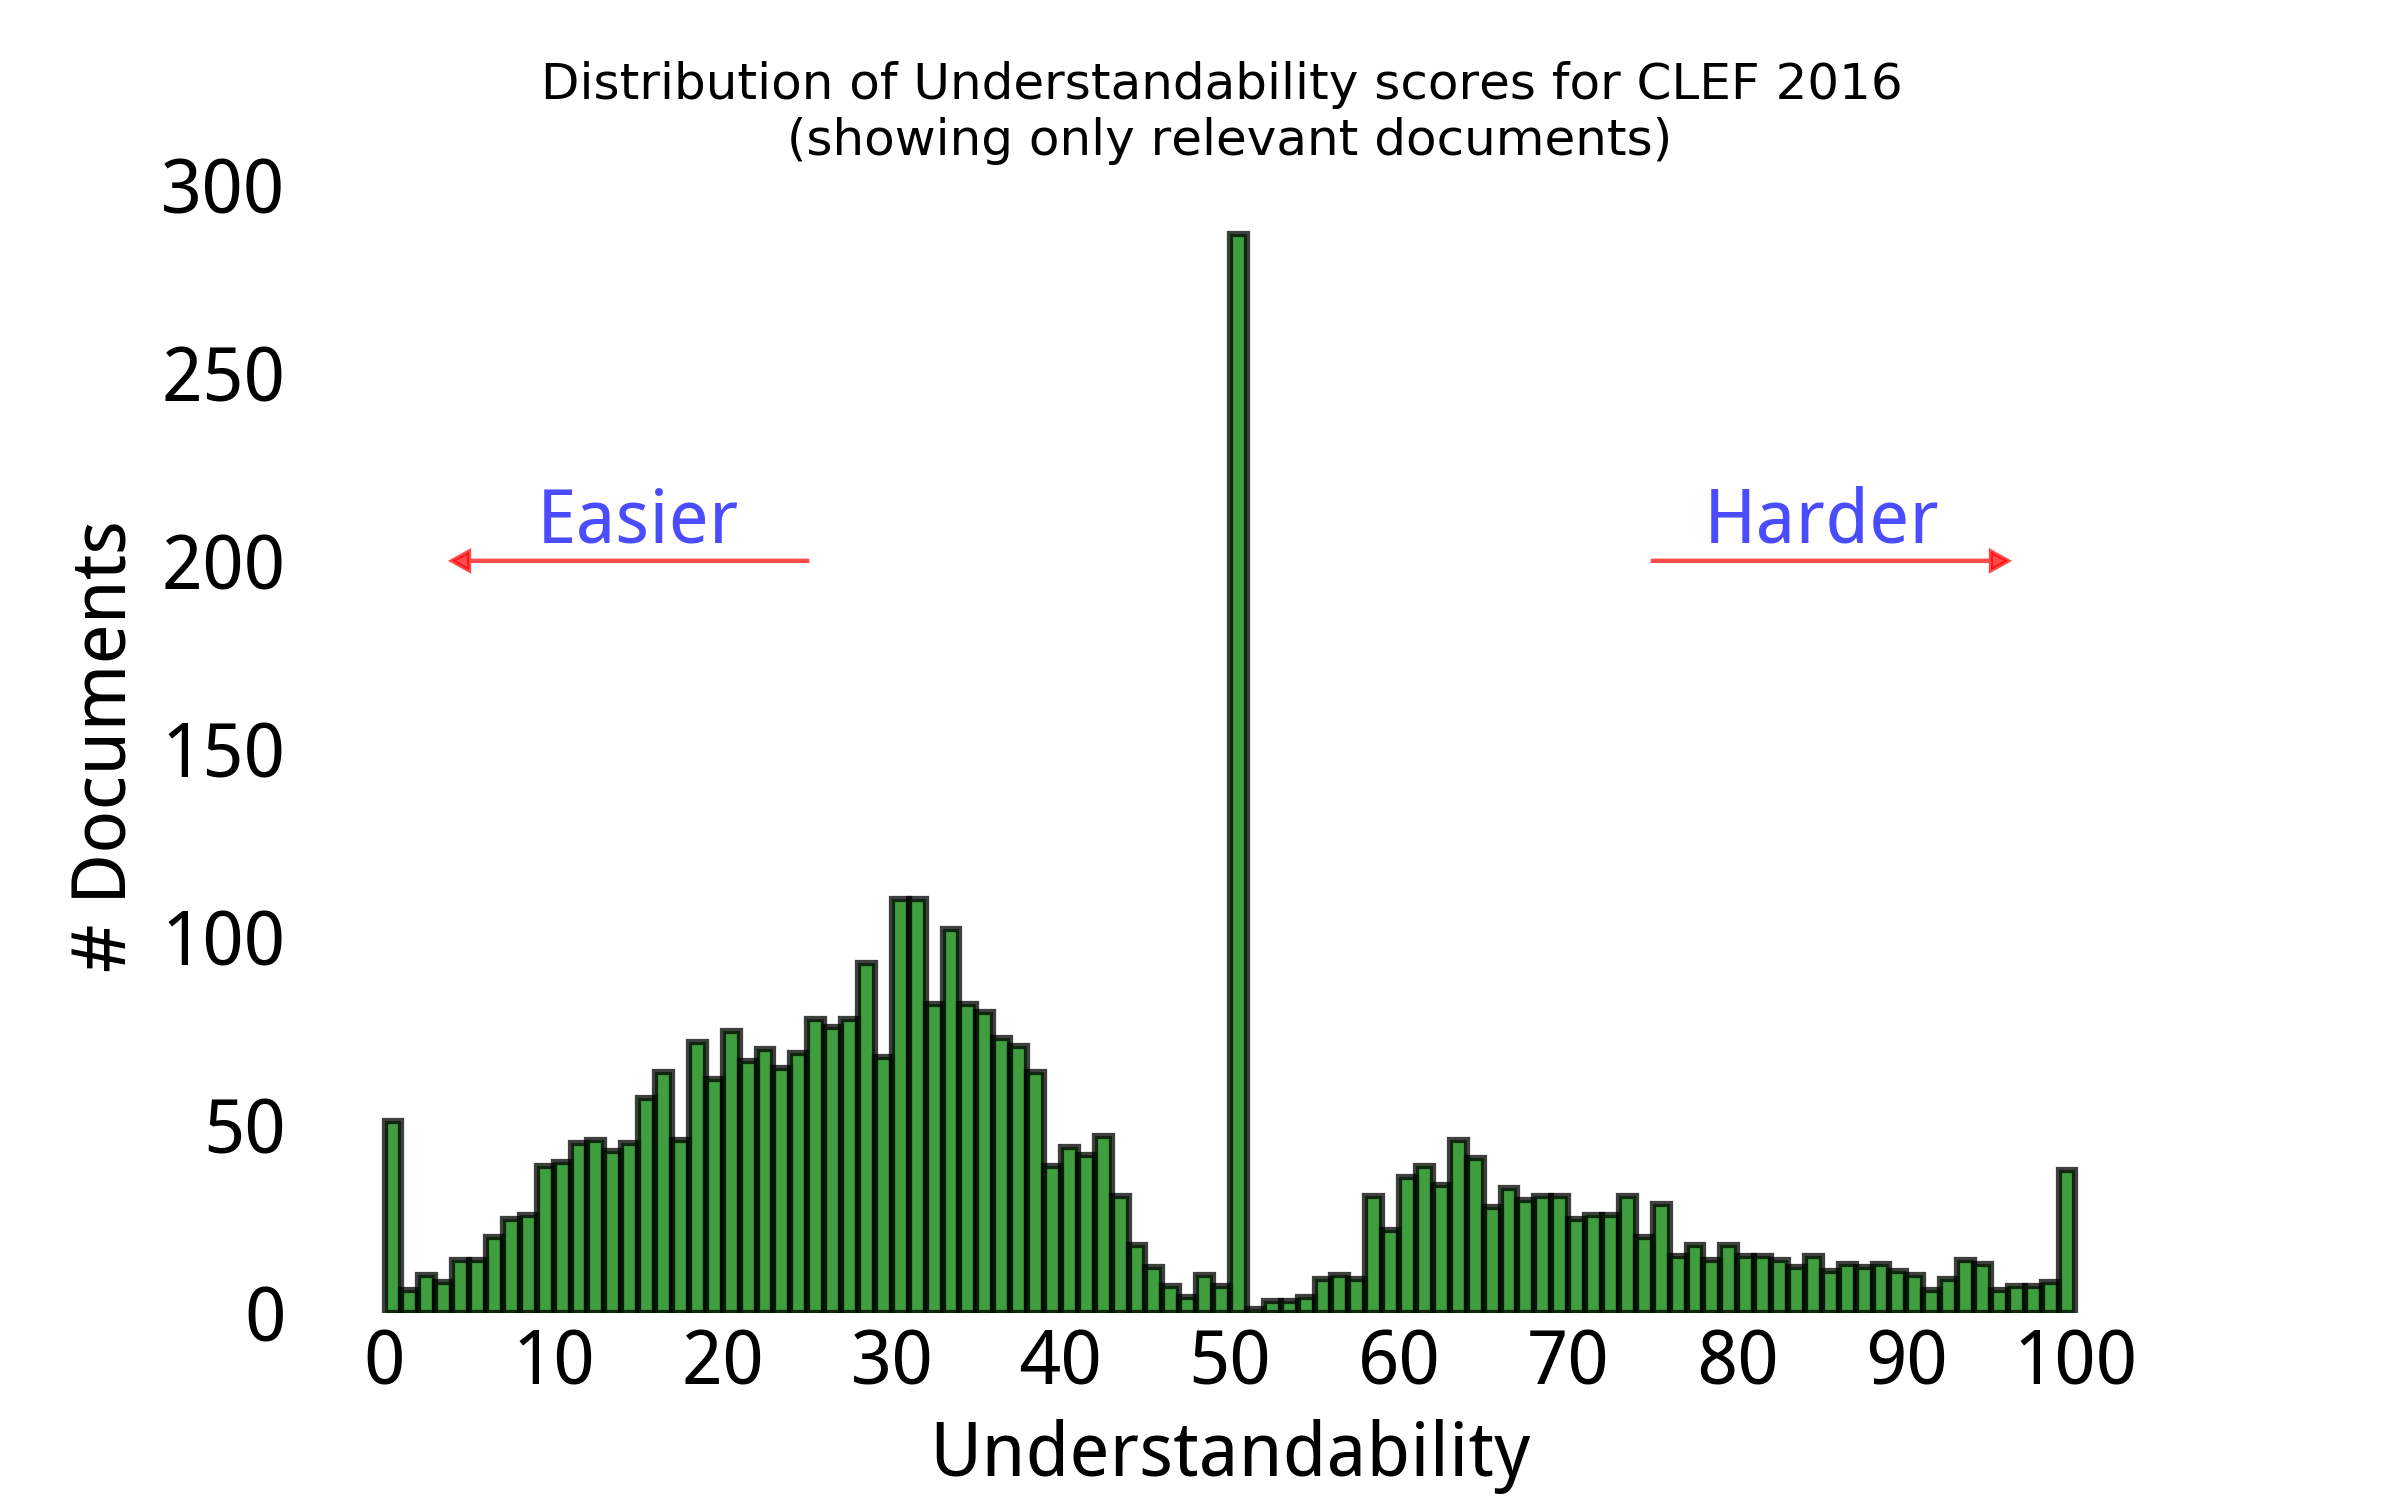
\includegraphics[width=0.8\textwidth]{appendix/hist_unders16.png}
    \caption{Understandability label distribution for CLEF eHealth 2016}
	\label{fig:dist}
\end{figure}

\begin{figure}[h!]
	\centering
	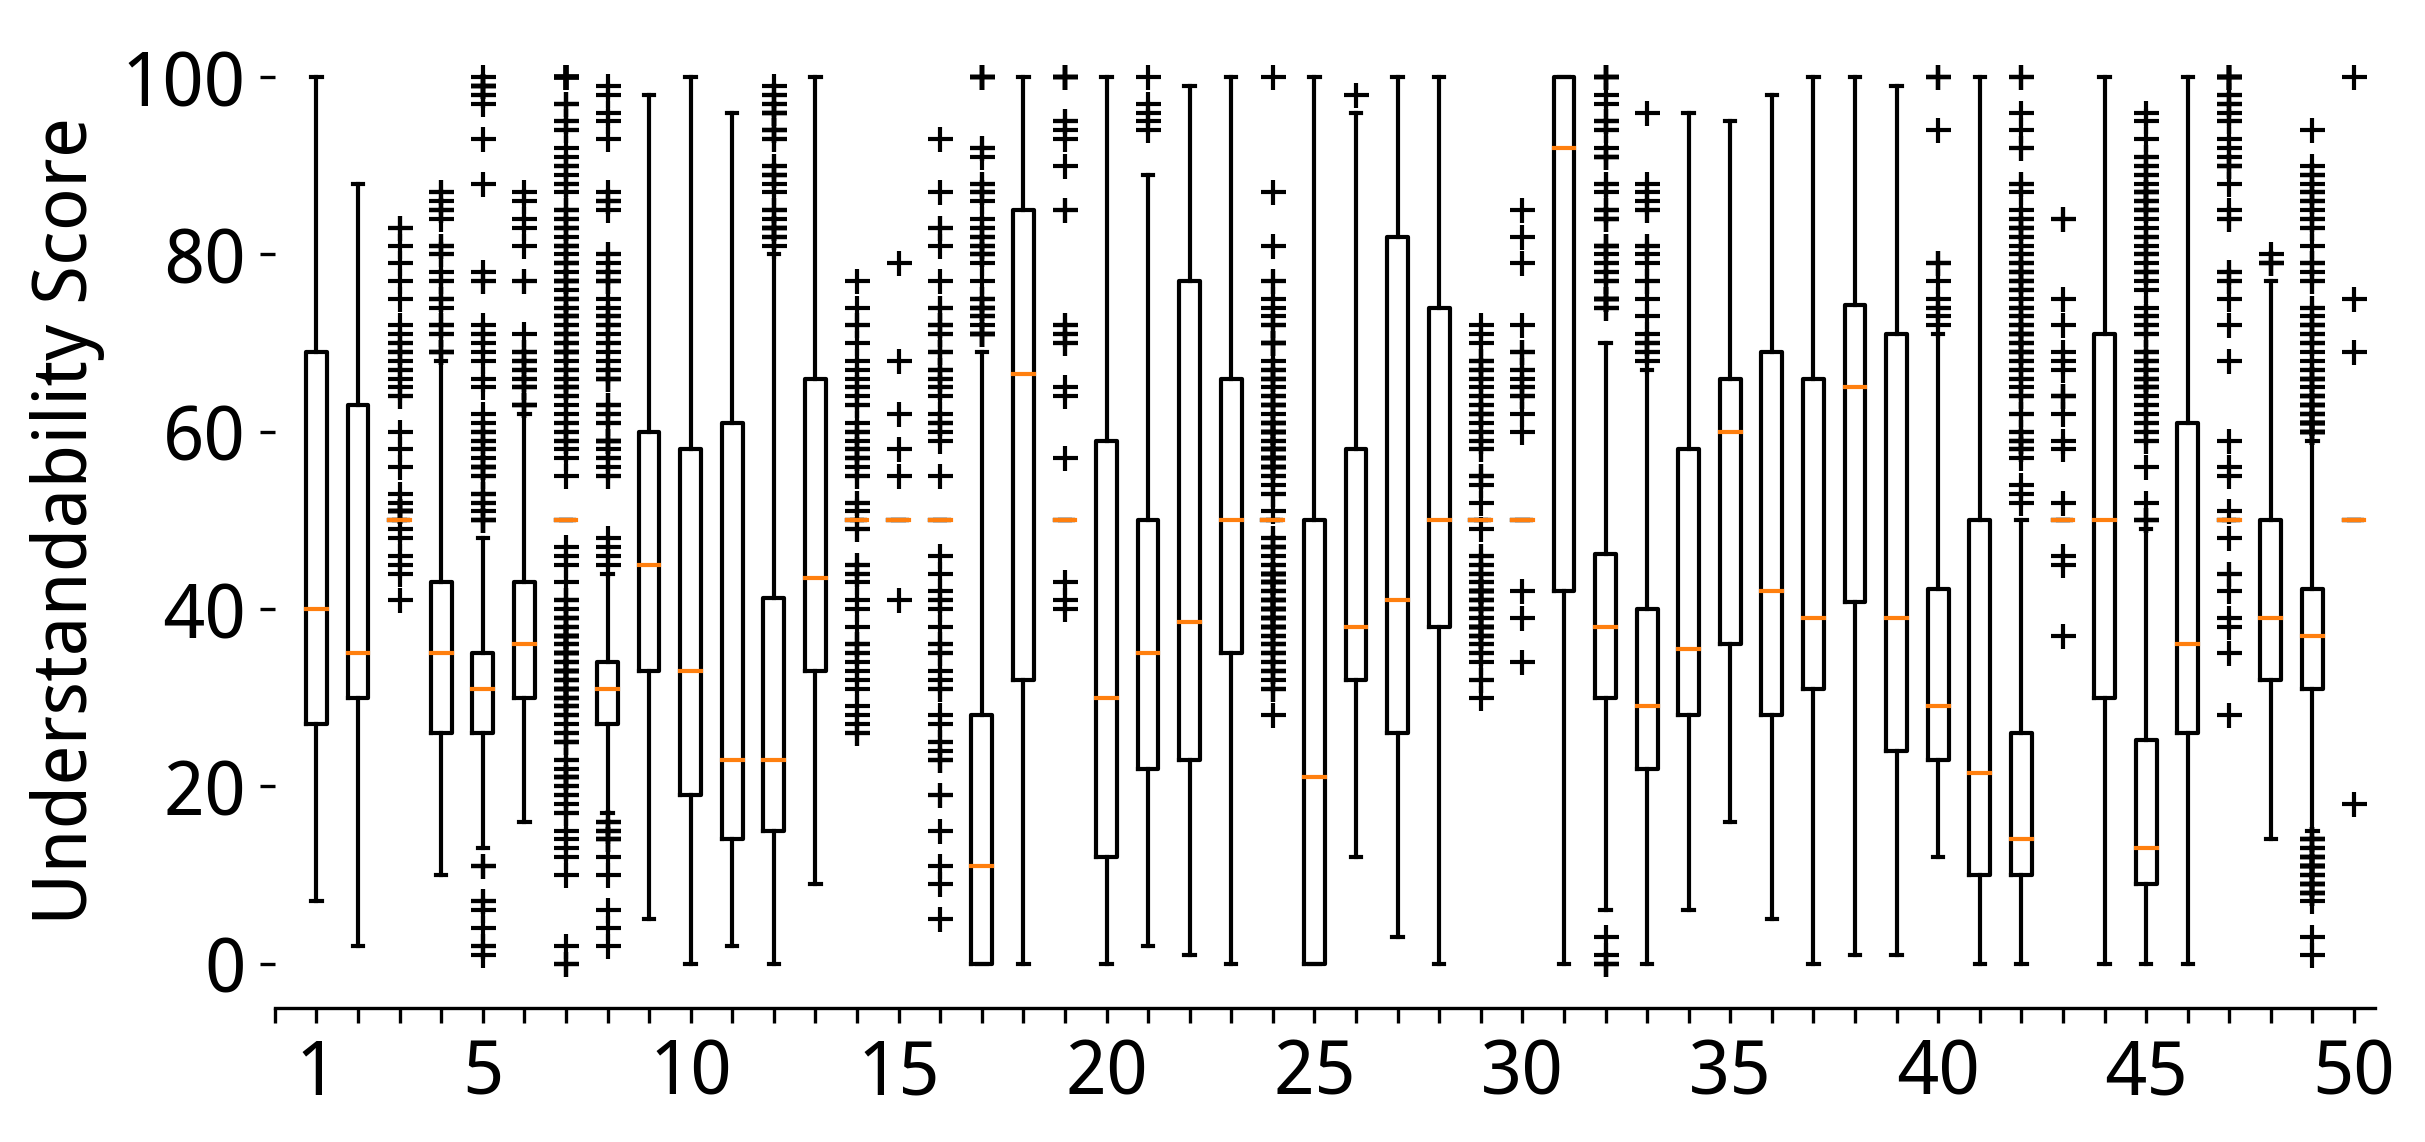
\includegraphics[width=.8\textwidth]{appendix/unders_per_topic_clef16.png}
    \caption{Understandability distribution broken per topic for CLEF eHealth 2016}
	\label{fig:dist}
\end{figure}


% Comparison with our CIKM short paper.
\begin{figure}[h!]
	\centering
	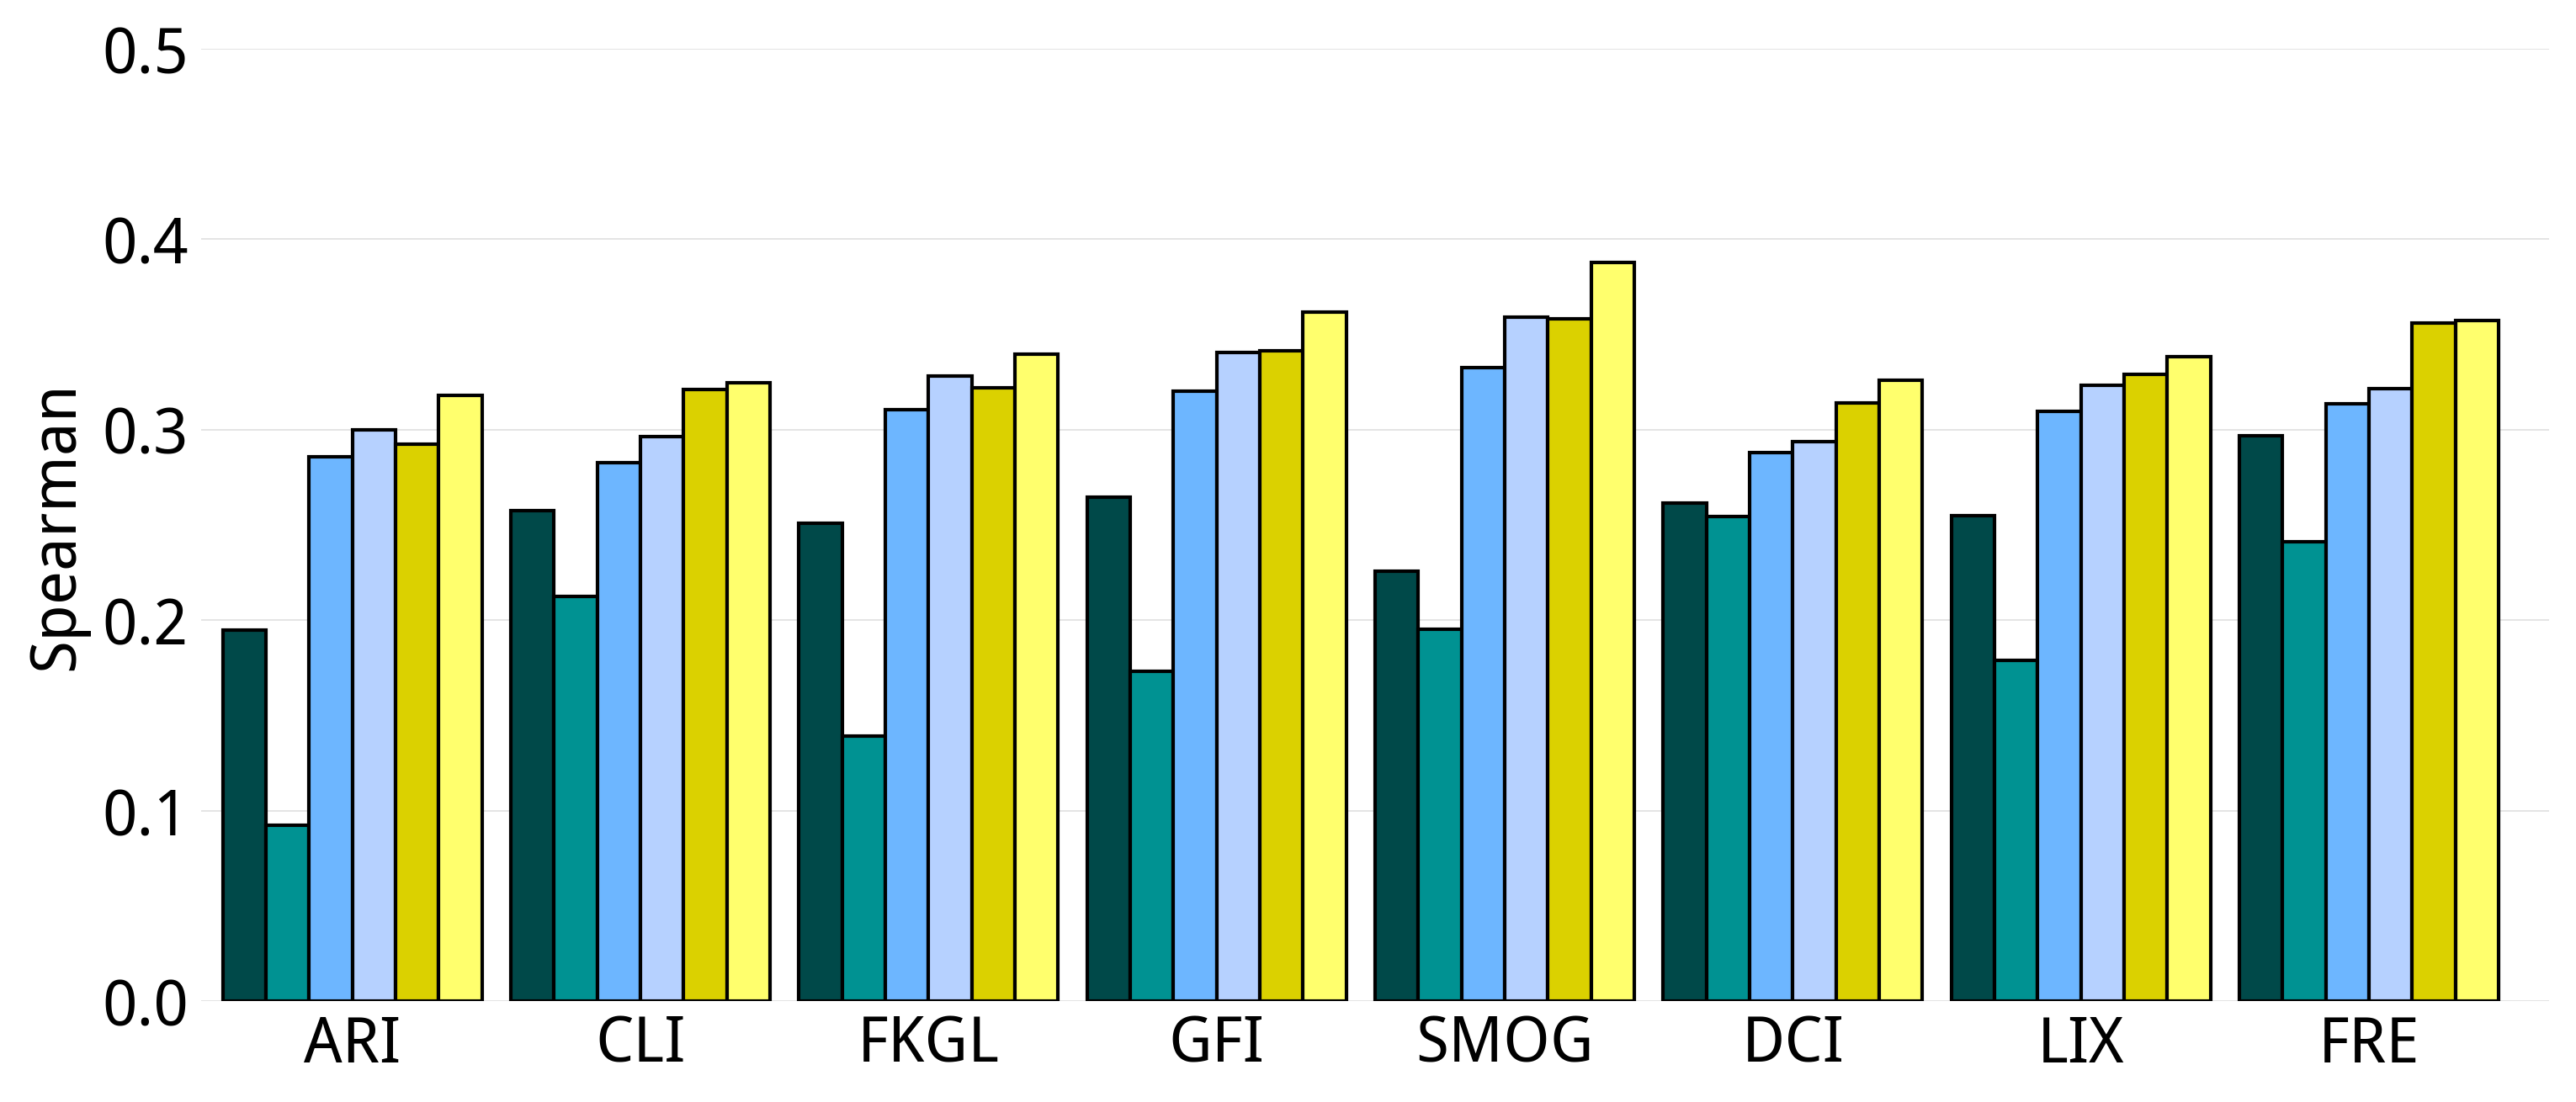
\includegraphics[width=.6\textwidth]{appendix/bar_corr_spearman15_values}
	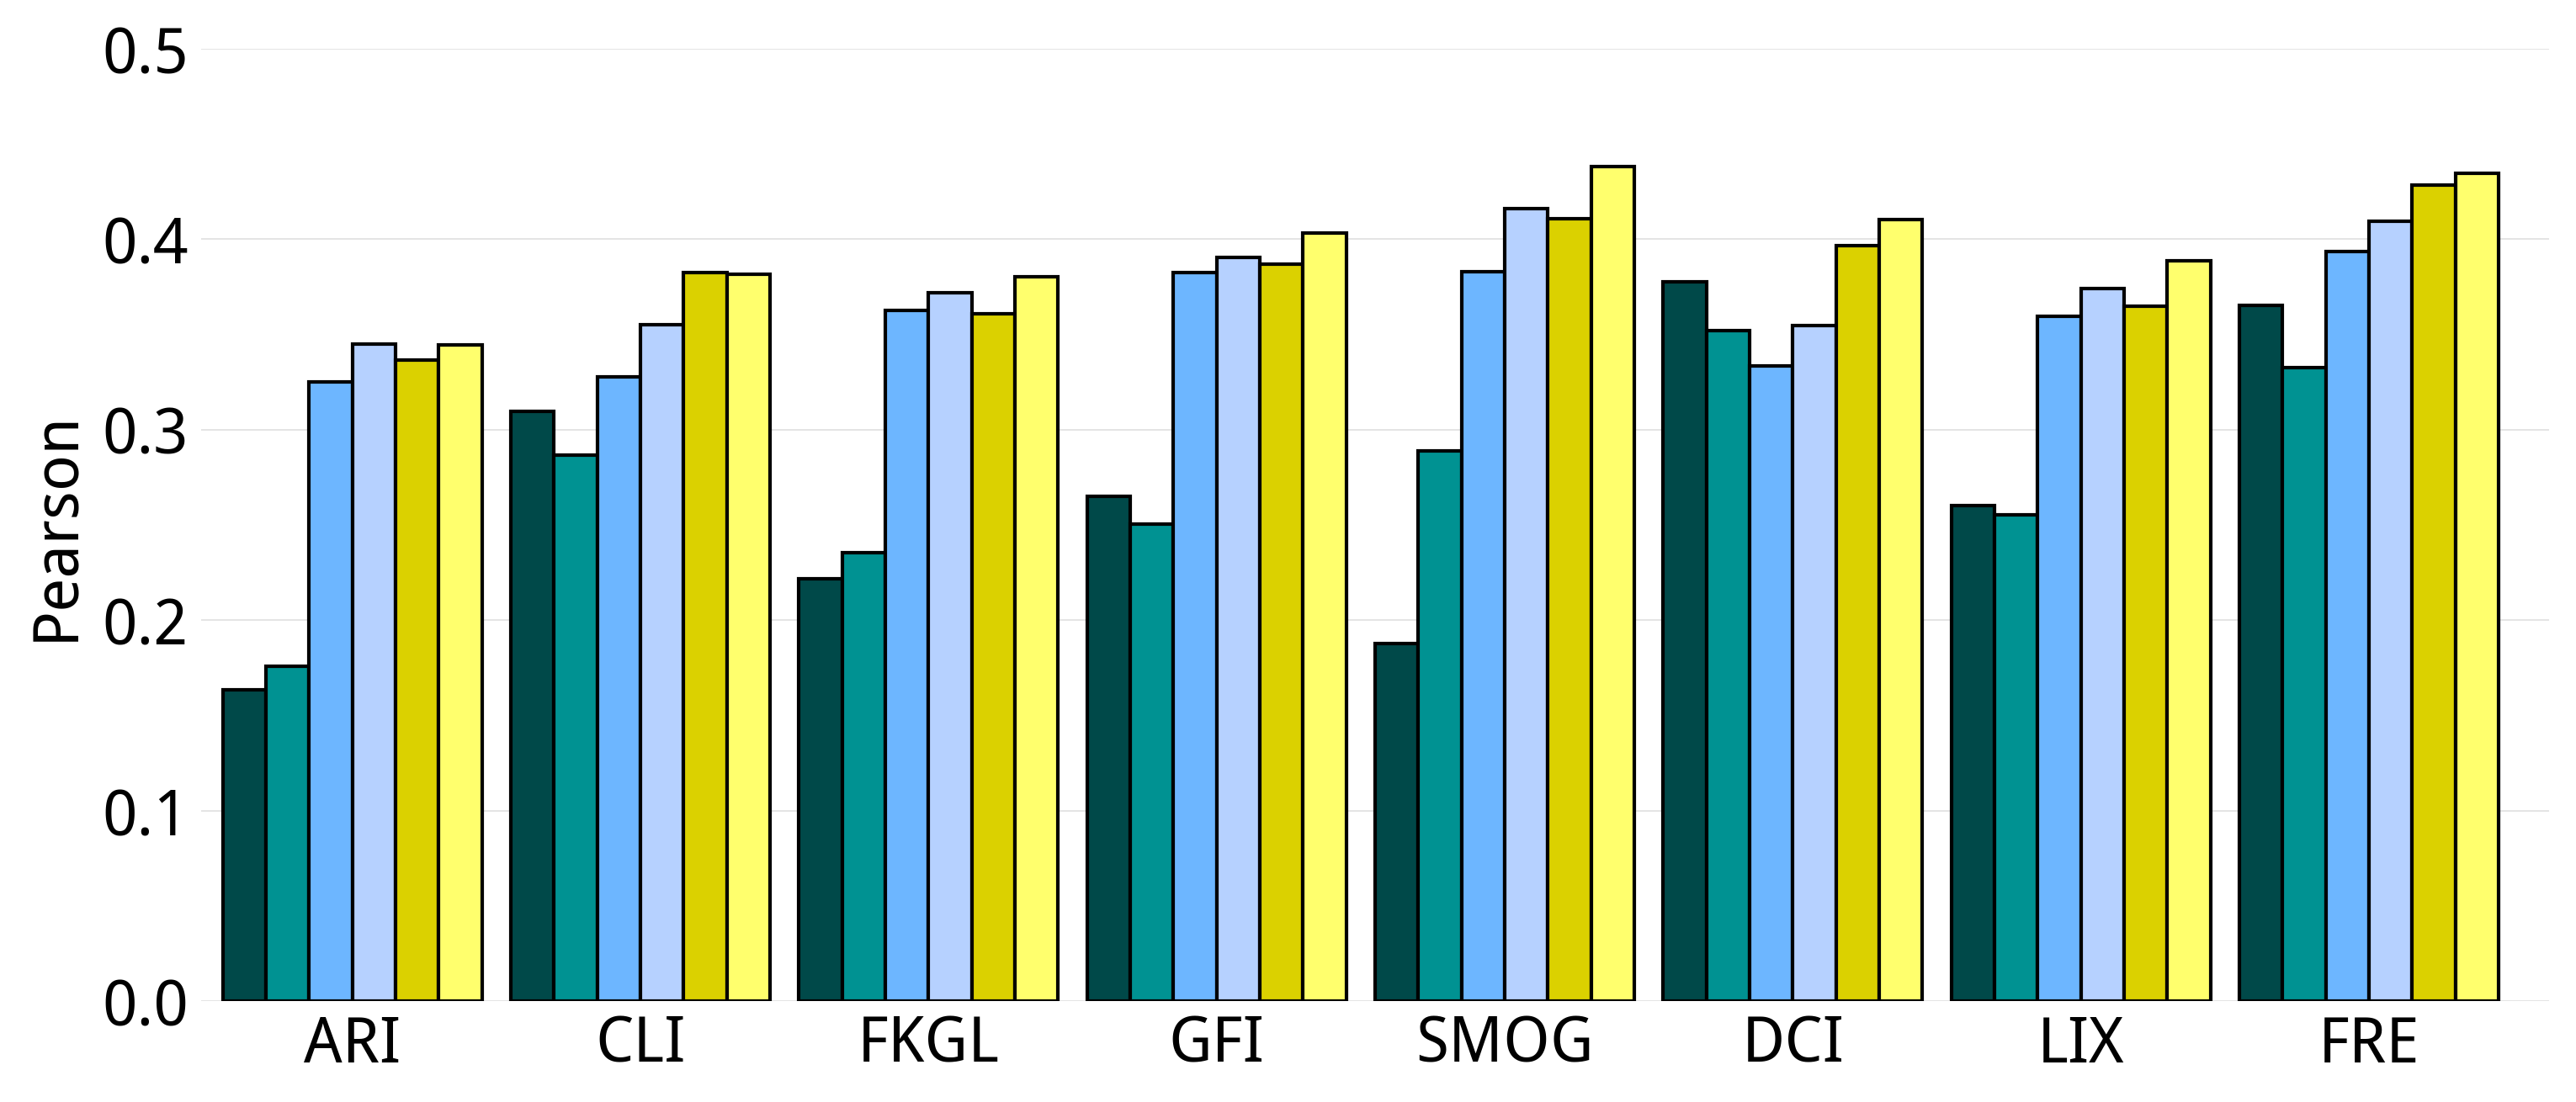
\includegraphics[width=.6\textwidth]{appendix/bar_corr_pearson15_values}
	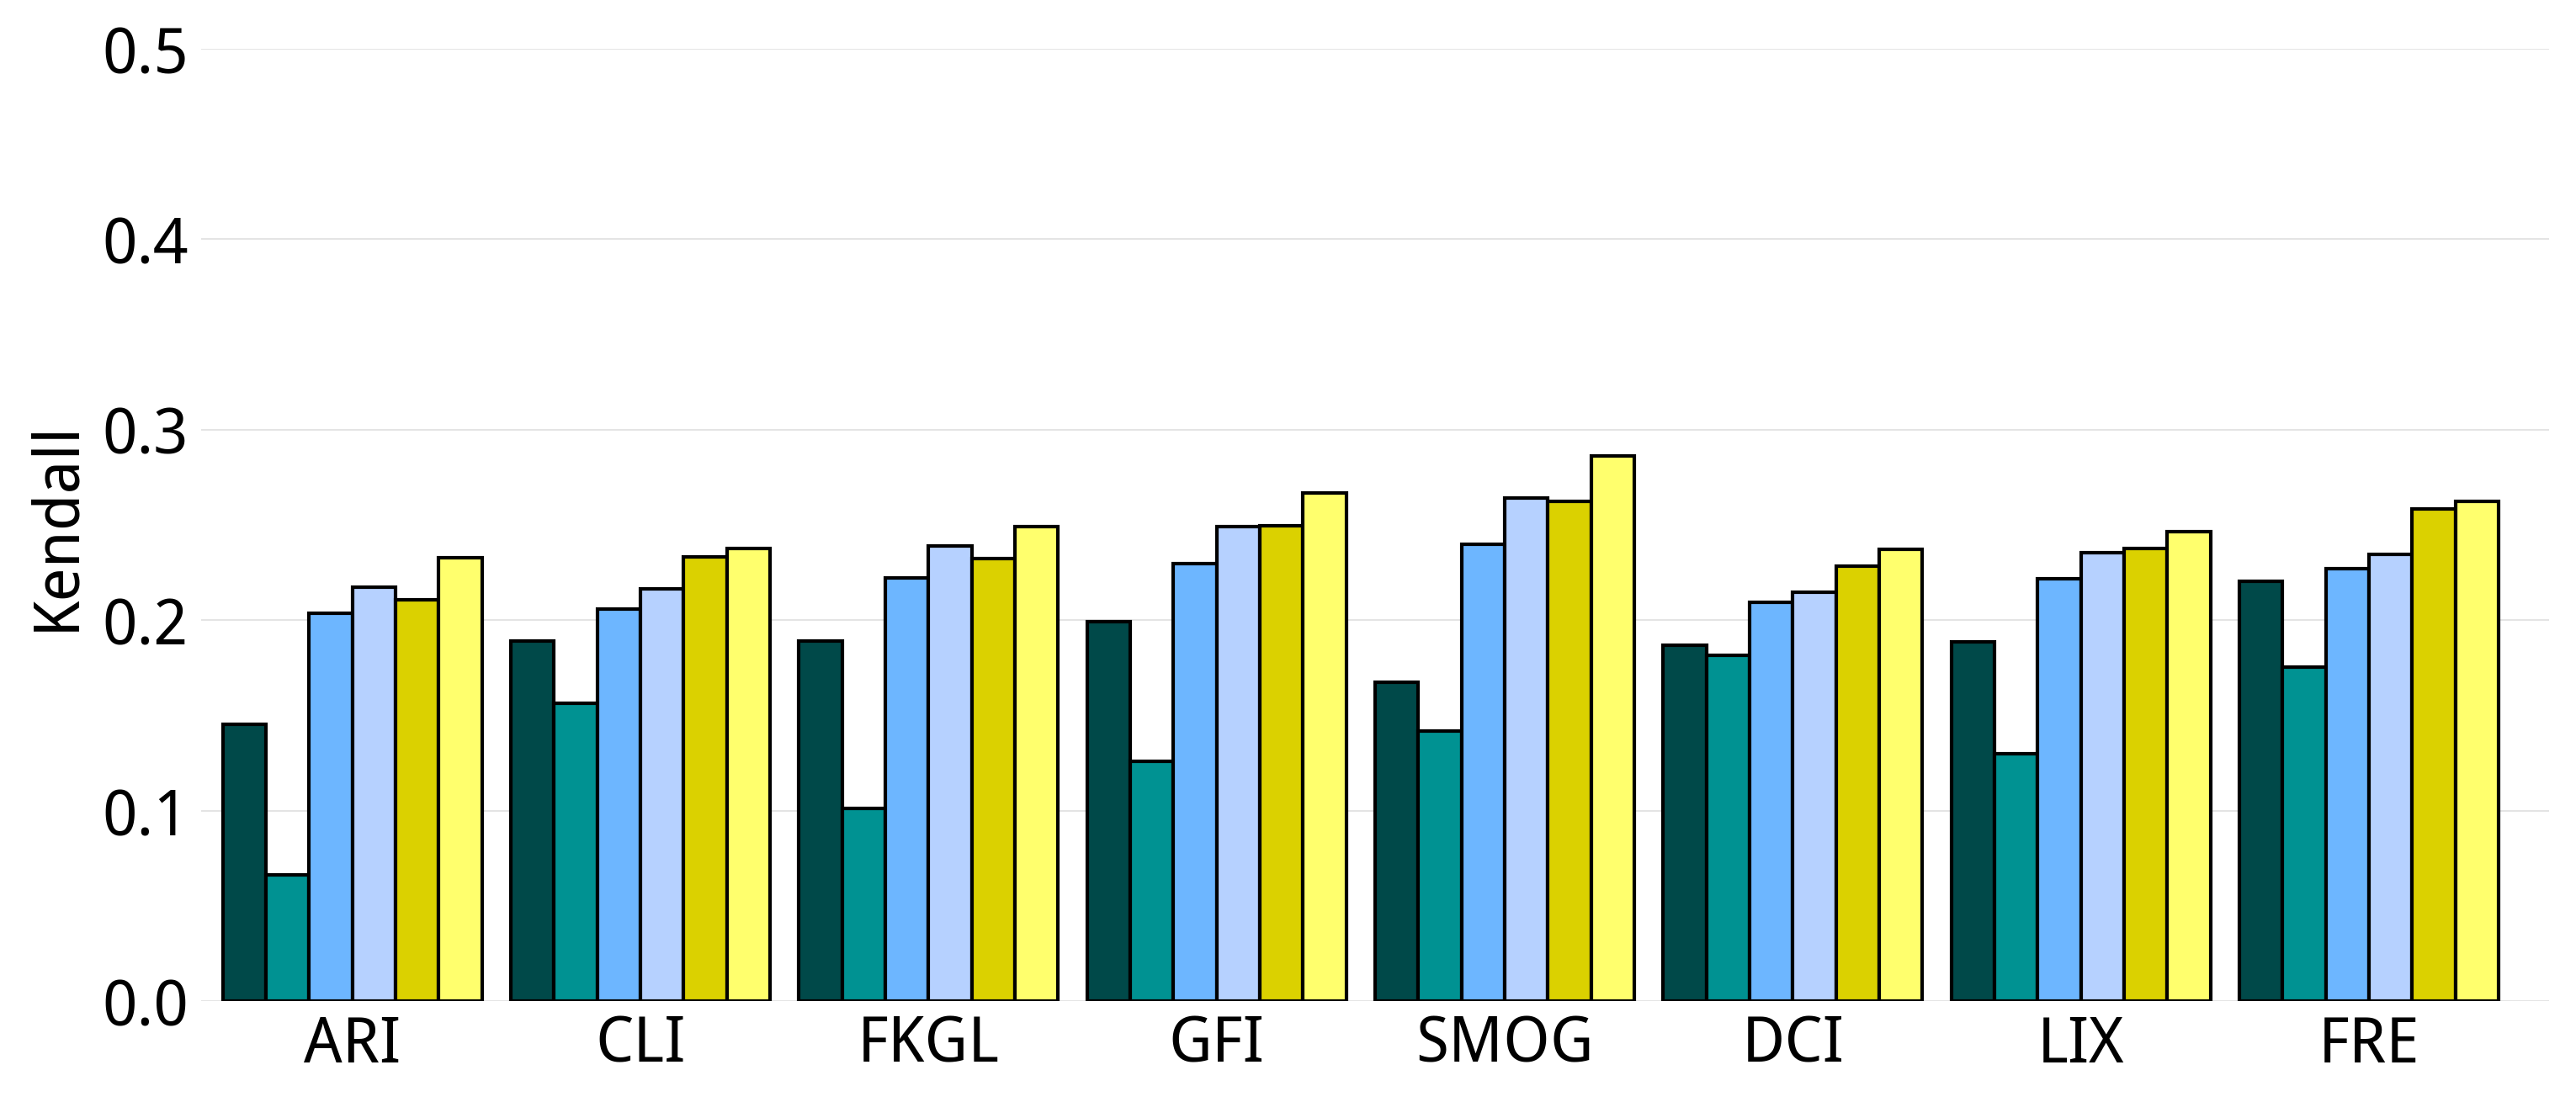
\includegraphics[width=.6\textwidth]{appendix/bar_corr_kendalltau15_values}
	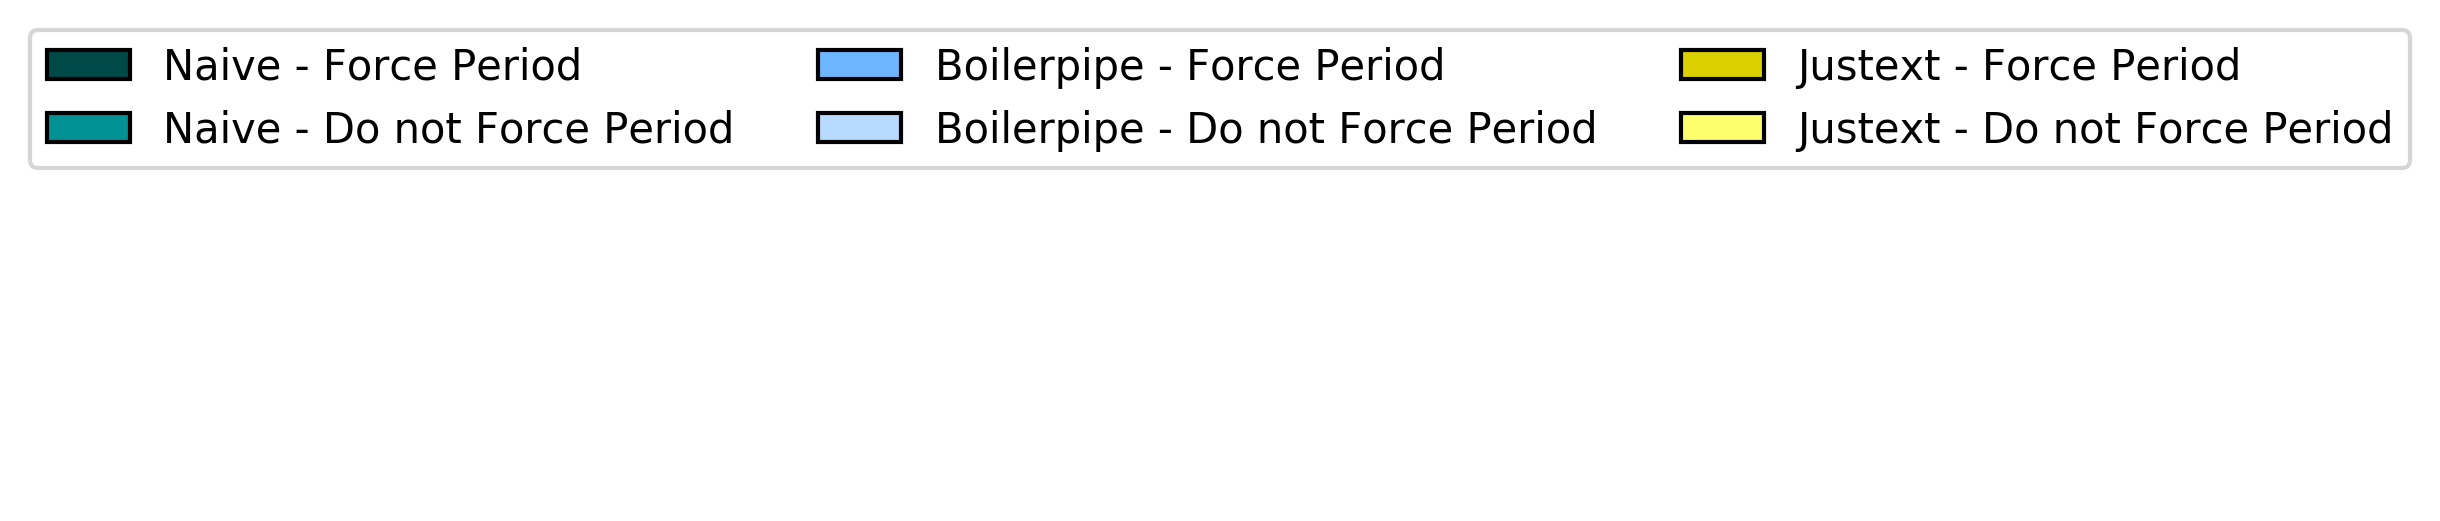
\includegraphics[width=.6\textwidth]{appendix/bar_raw_values}
    \caption{In Palotti et al.~\cite{palotti15}, authors investigates the influence of HTML preprocessing when readability formulas are used to estimate Webpage understandability. They found that readability formulas are heavily affected by the methods used to extract text from the HTML source, but they did not measure how correlated each method was with a human ground truth. We further extended Palotti et al.'s work to understand the influence of HTML preprocessing on automatic understandability methods and establish best practices. We show the correlation of each preprocessing combination with the ground truth assessments for \textbf{CLEF 2015}.}
	\label{fig:dist}
\end{figure}

\begin{figure}[h!]
	\centering
	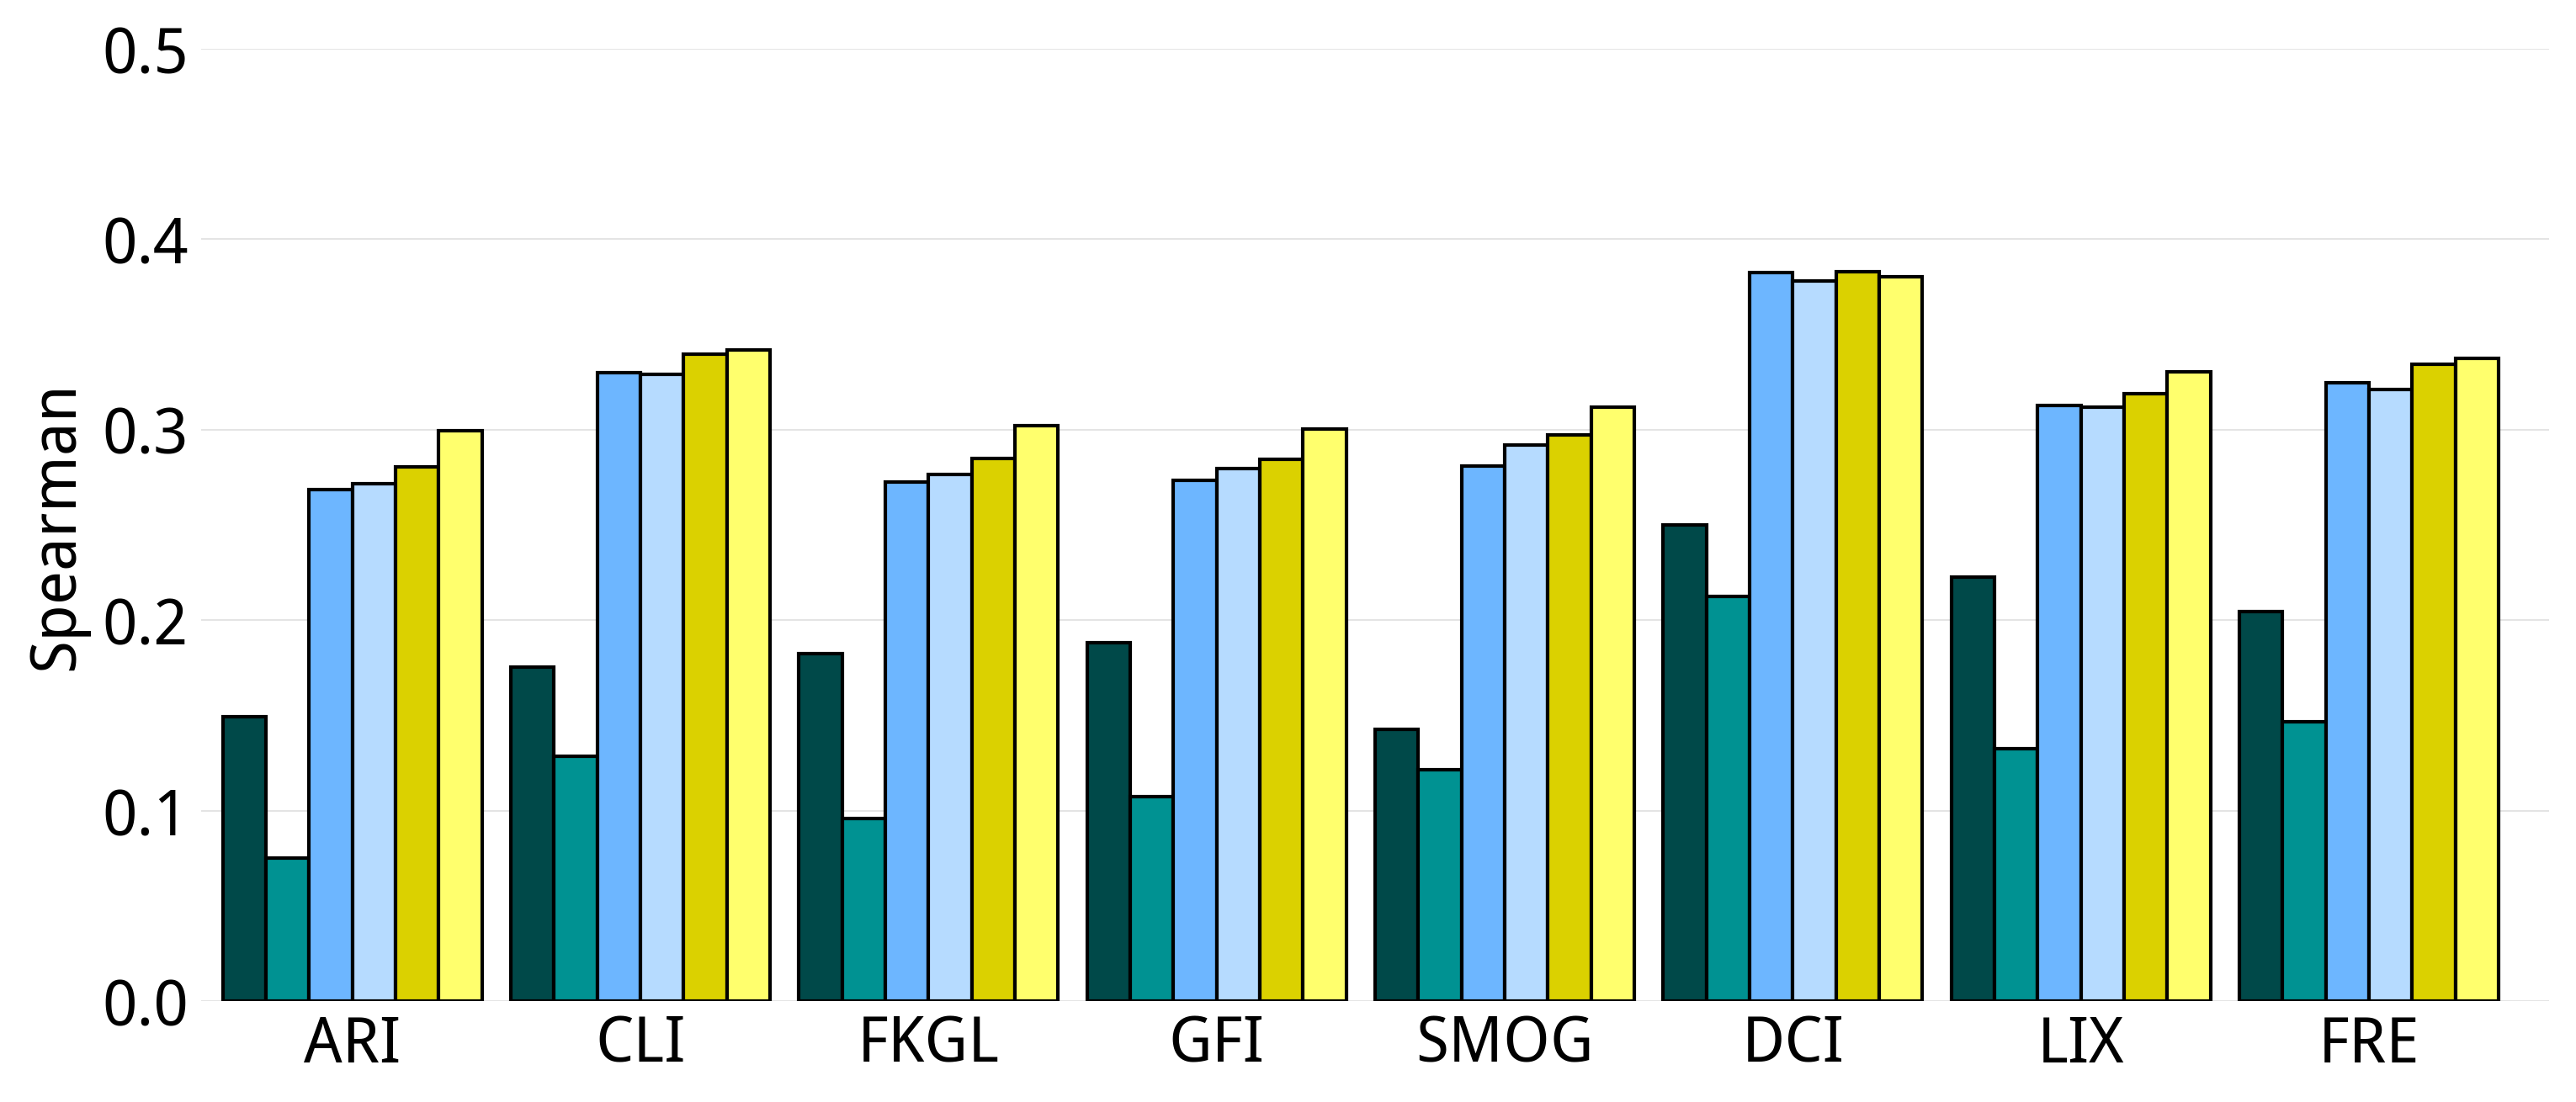
\includegraphics[width=.6\textwidth]{appendix/bar_corr_spearman16_values}
	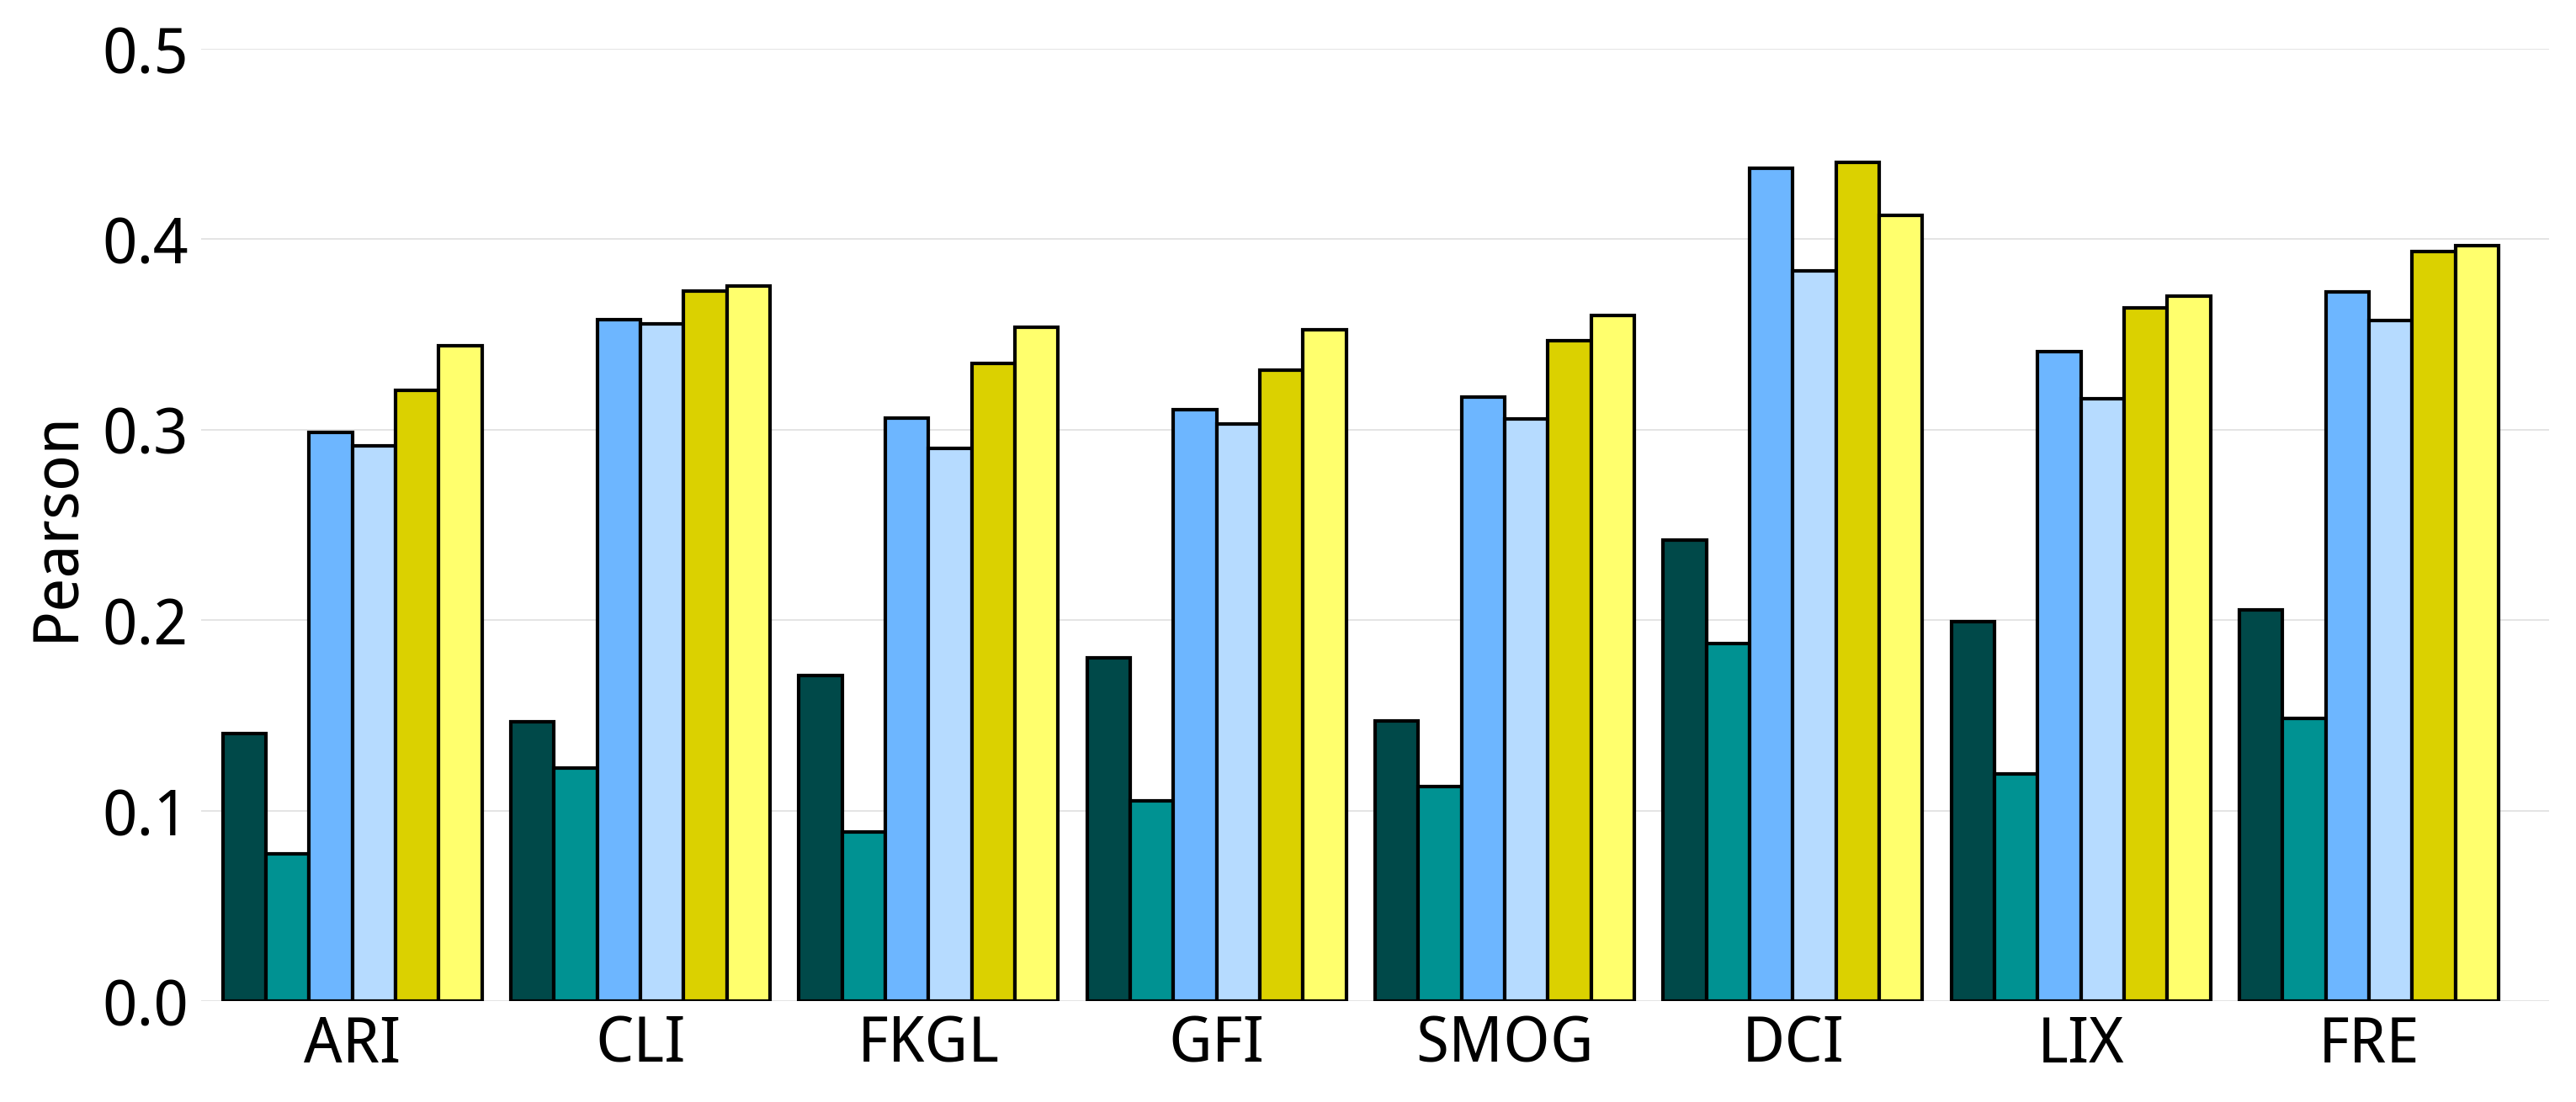
\includegraphics[width=.6\textwidth]{appendix/bar_corr_pearson16_values}
	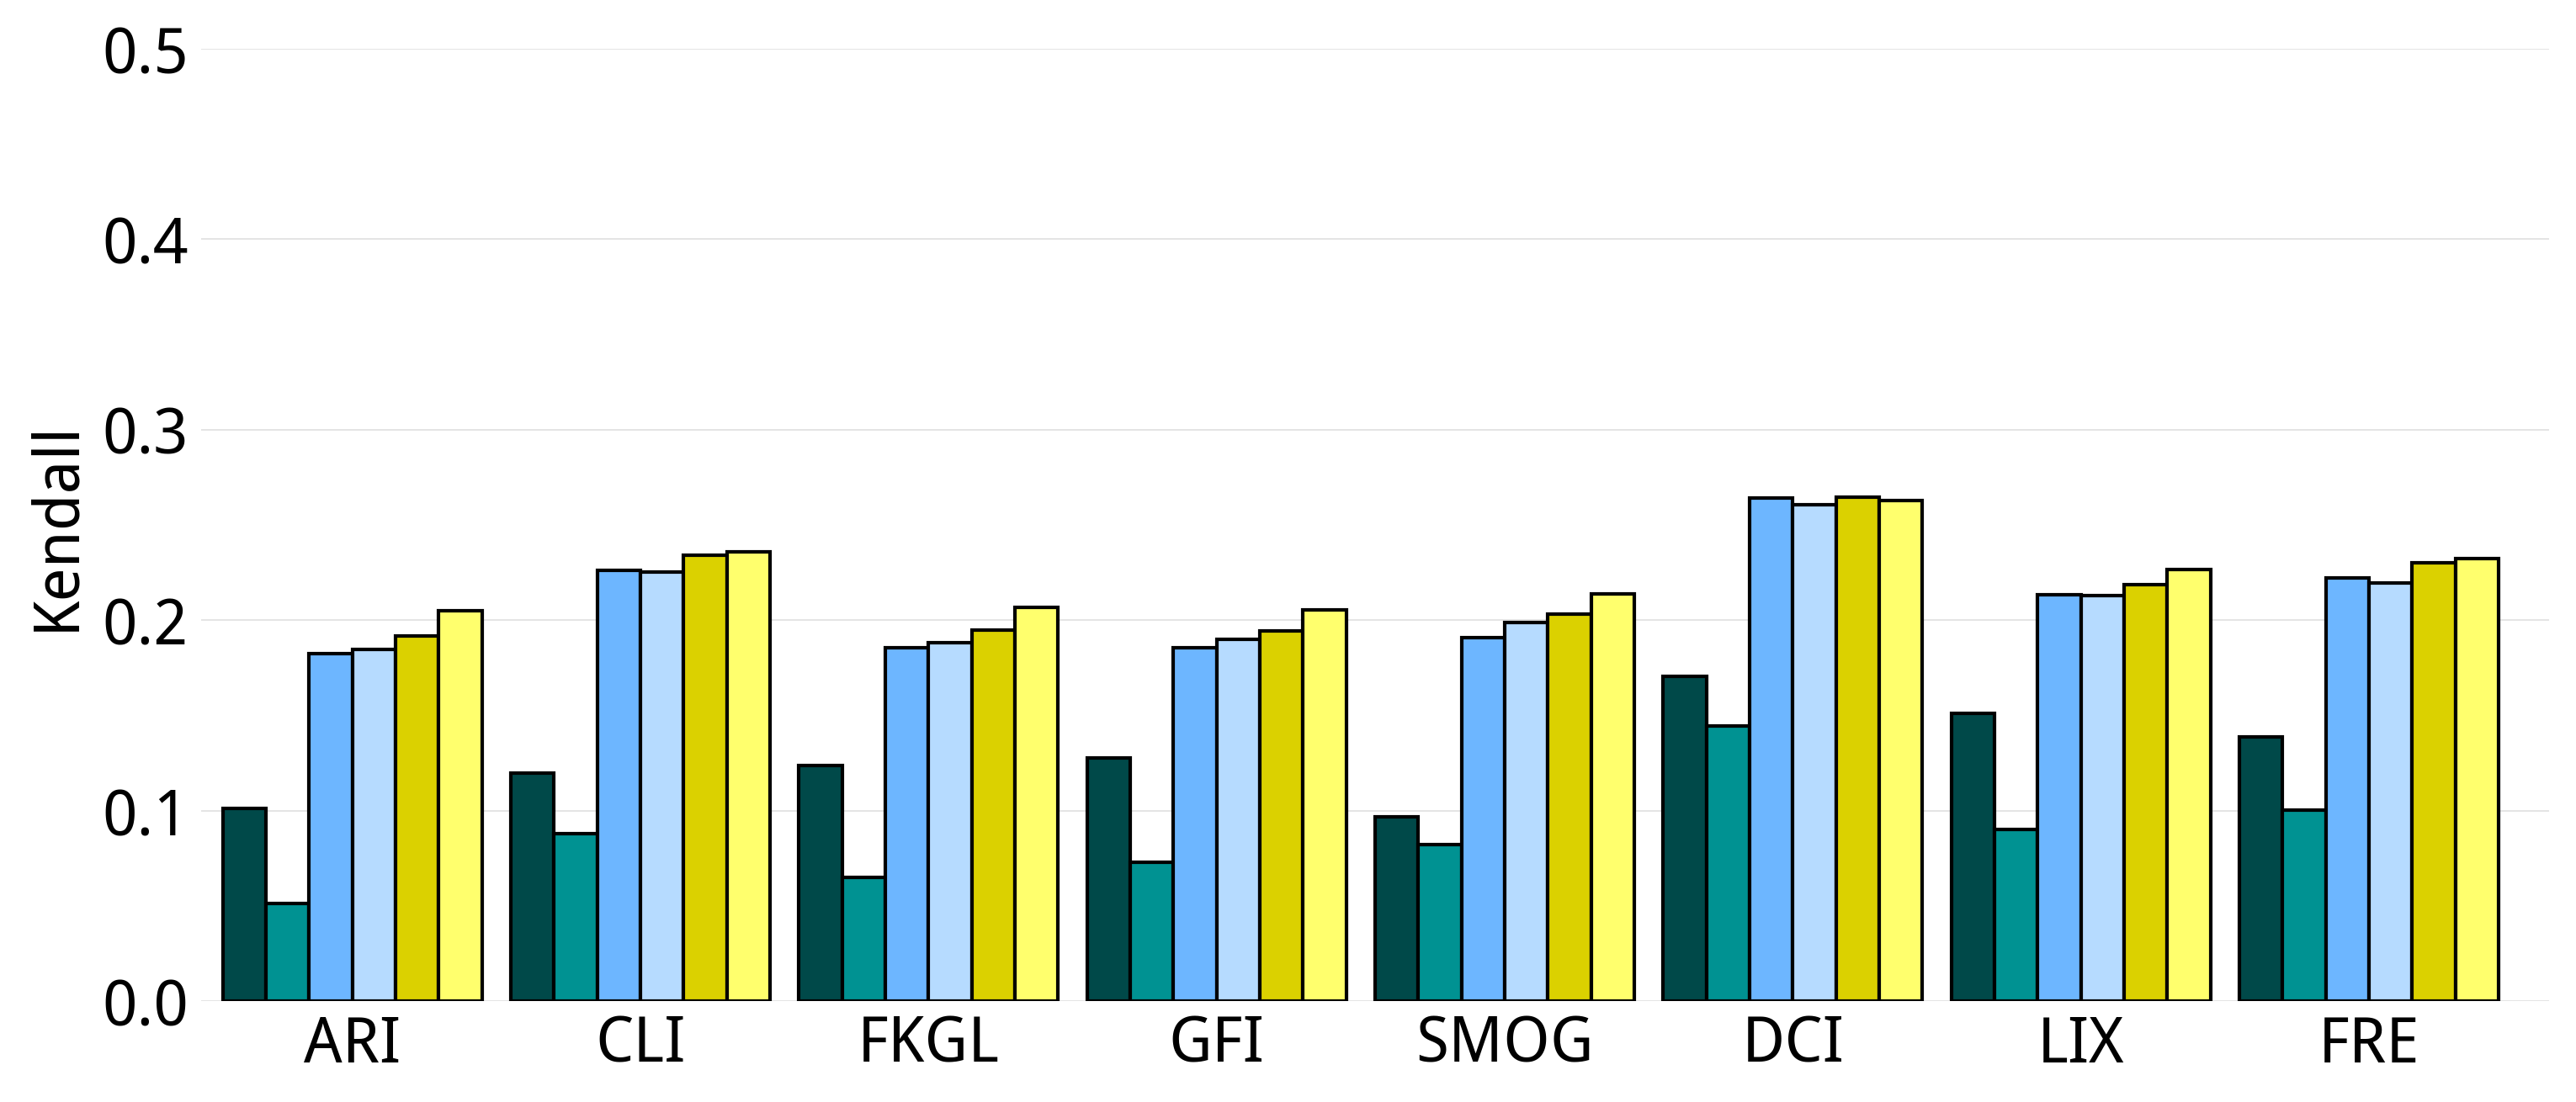
\includegraphics[width=.6\textwidth]{appendix/bar_corr_kendalltau16_values}
	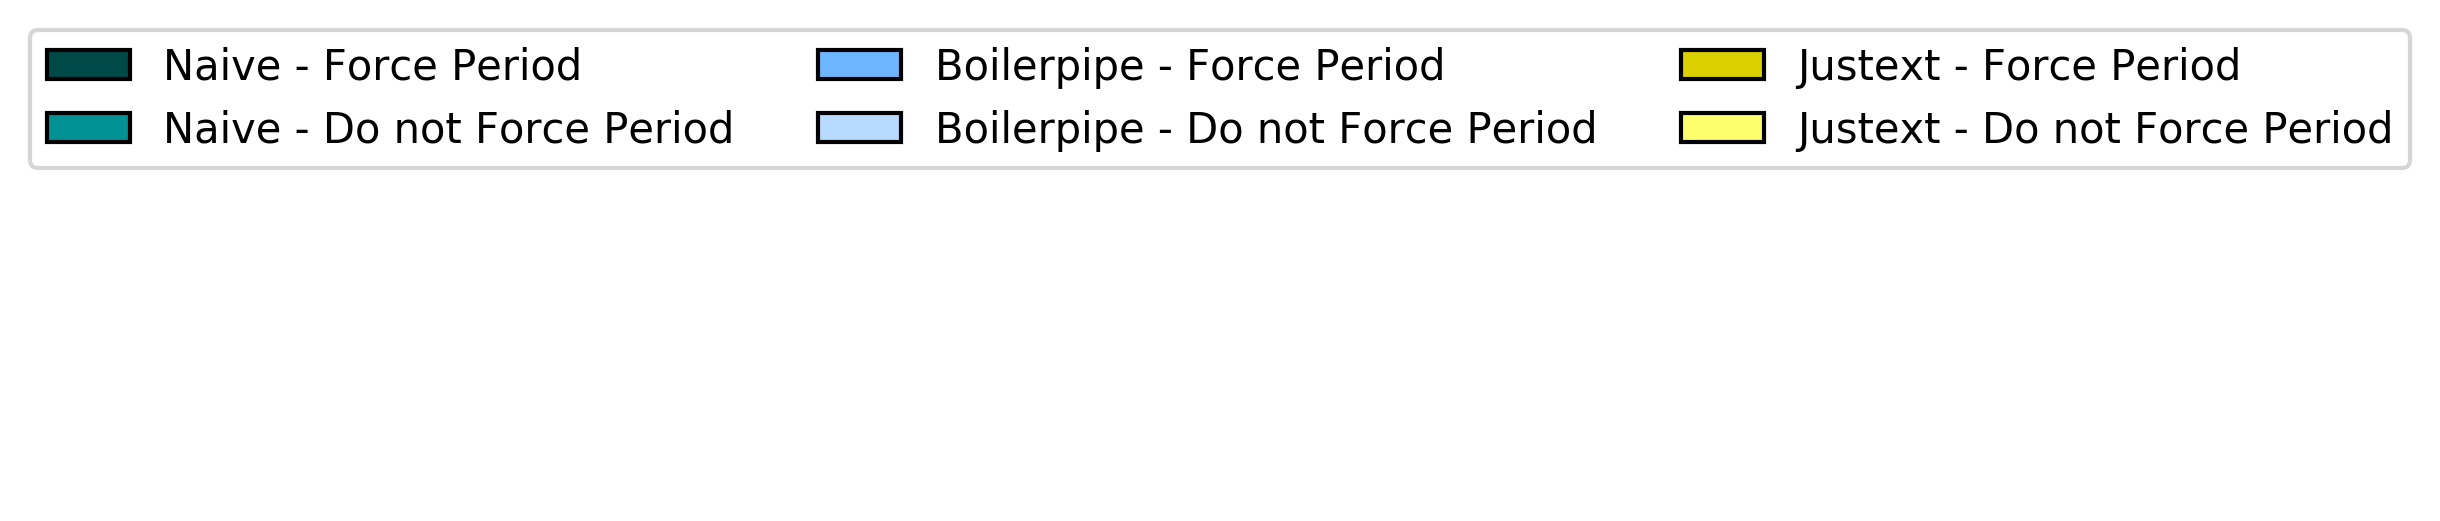
\includegraphics[width=.6\textwidth]{appendix/bar_raw_values}
    \caption{In Palotti et al.~\cite{palotti15}, authors investigates the influence of HTML preprocessing when readability formulas are used to estimate Webpage understandability. They found that readability formulas are heavily affected by the methods used to extract text from the HTML source, but they did not measure how correlated each method was with a human ground truth. We further extended Palotti et al.'s work to understand the influence of HTML preprocessing on automatic understandability methods and establish best practices. We show the correlation of each preprocessing combination with the ground truth assessments for \textbf{CLEF 2016}.}
	\label{fig:dist}
\end{figure}


%%%% Pearson and kendalltau correlation. In the paper, we show only the spearman one.

\begin{figure}[h!]
	\centering
	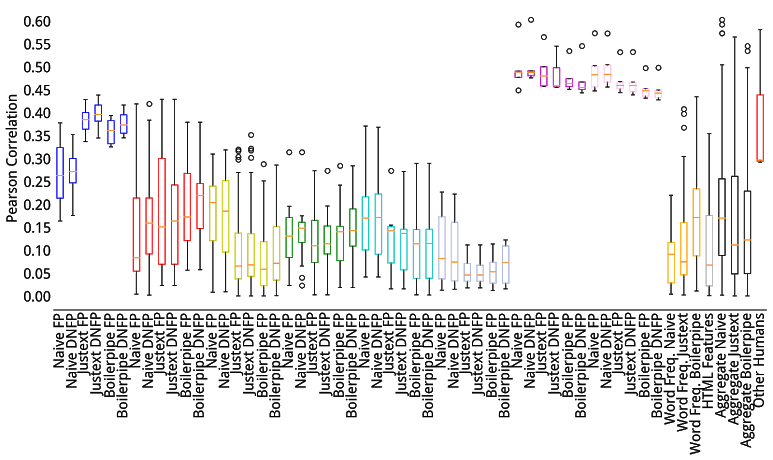
\includegraphics[width=.6\textwidth]{appendix/box_pearson15_raw_values}
    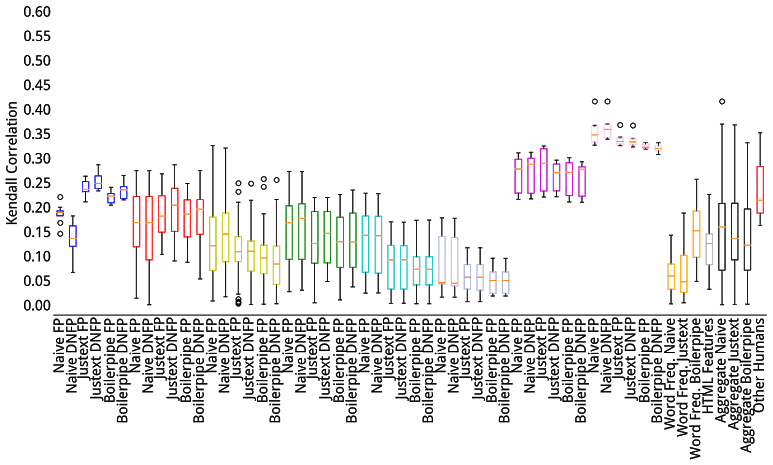
\includegraphics[width=.6\textwidth]{appendix/box_kendalltau15_raw_values}
	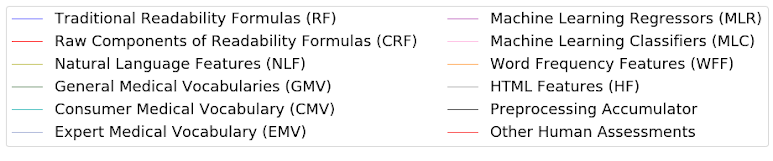
\includegraphics[width=.6\textwidth]{appendix/legendCorr}
    \caption{Correlations between understandability estimators and human assessments for \textbf{CLEF 2015}.}
	\label{fig:dist}
\end{figure}

\begin{figure}[h!]
	\centering
	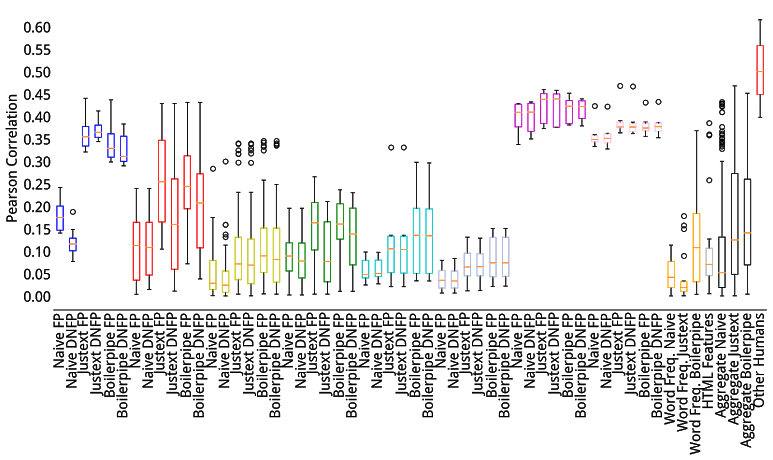
\includegraphics[width=.6\textwidth]{appendix/box_pearson16_raw_values}
    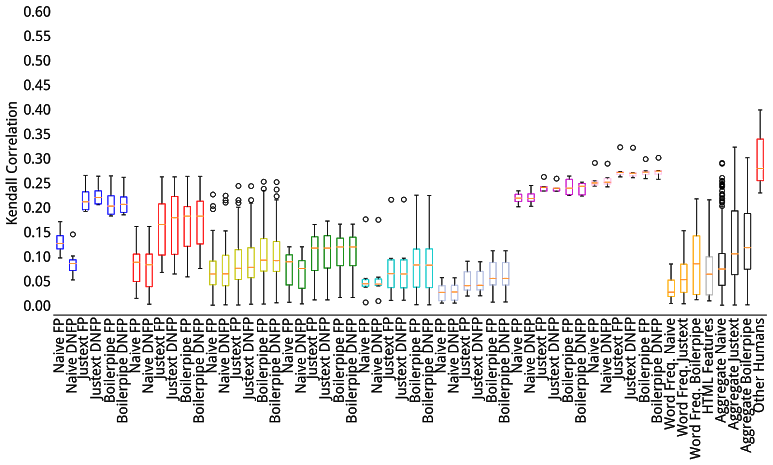
\includegraphics[width=.6\textwidth]{appendix/box_kendalltau16_raw_values}
	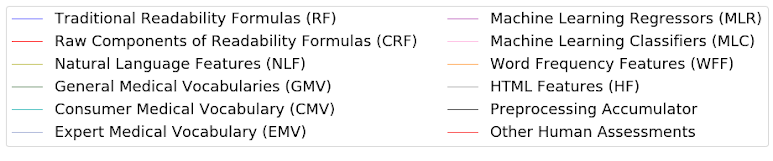
\includegraphics[width=.6\textwidth]{appendix/legendCorr}
    \caption{Correlations between understandability estimators and human assessments for \textbf{CLEF 2015}.}
	\label{fig:dist}
\end{figure}


\begin{figure}[h!]
	\centering
	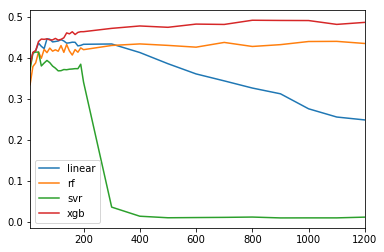
\includegraphics[width=.6\textwidth]{appendix/features}
    \caption{To study the impact of feature sets, we varied the number of features each regressor algorithm was trained with. For that, we selected features with Python's f\_regression algorithm from Sklearn package. The eXtreme Gradient Boosting (XGB) and Random Forest Regressor were marginally influenced by the selection of features, therefore we used XGB with all features devised in our experiments.}
	\label{fig:dist}
\end{figure}

\begin{figure}[h!]
	\centering
	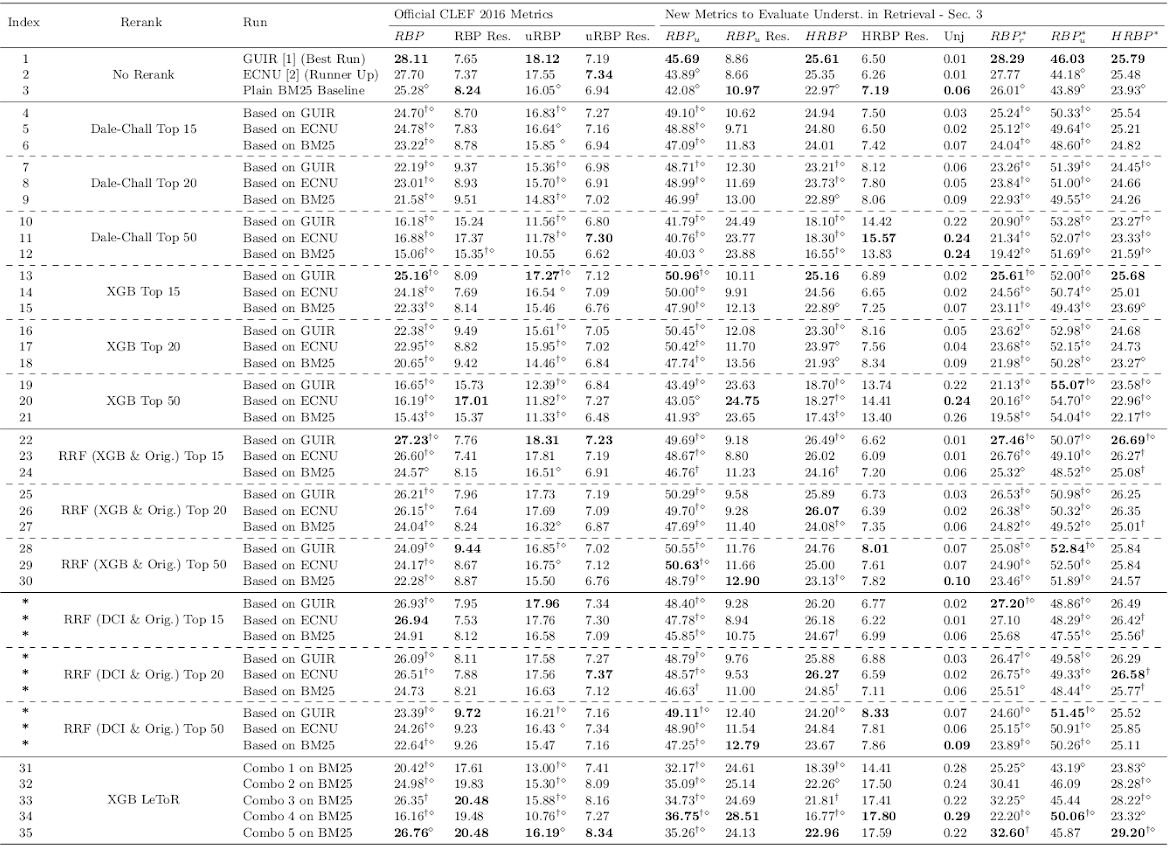
\includegraphics[width=1.0\textwidth]{appendix/tab_dci}
    \caption{We expanded retrieval results including the experiments with Reciprocal Rank Fusion (RRF) of Dale-Chall Index Runs (indices 4-12) and the original runs (indices 1-3). These results confirm the superiority of using XGB rather than DCI in terms of understandability of the results retrieved.}    
	\label{fig:dist}
\end{figure}

\begin{figure}[h!]
	\centering
	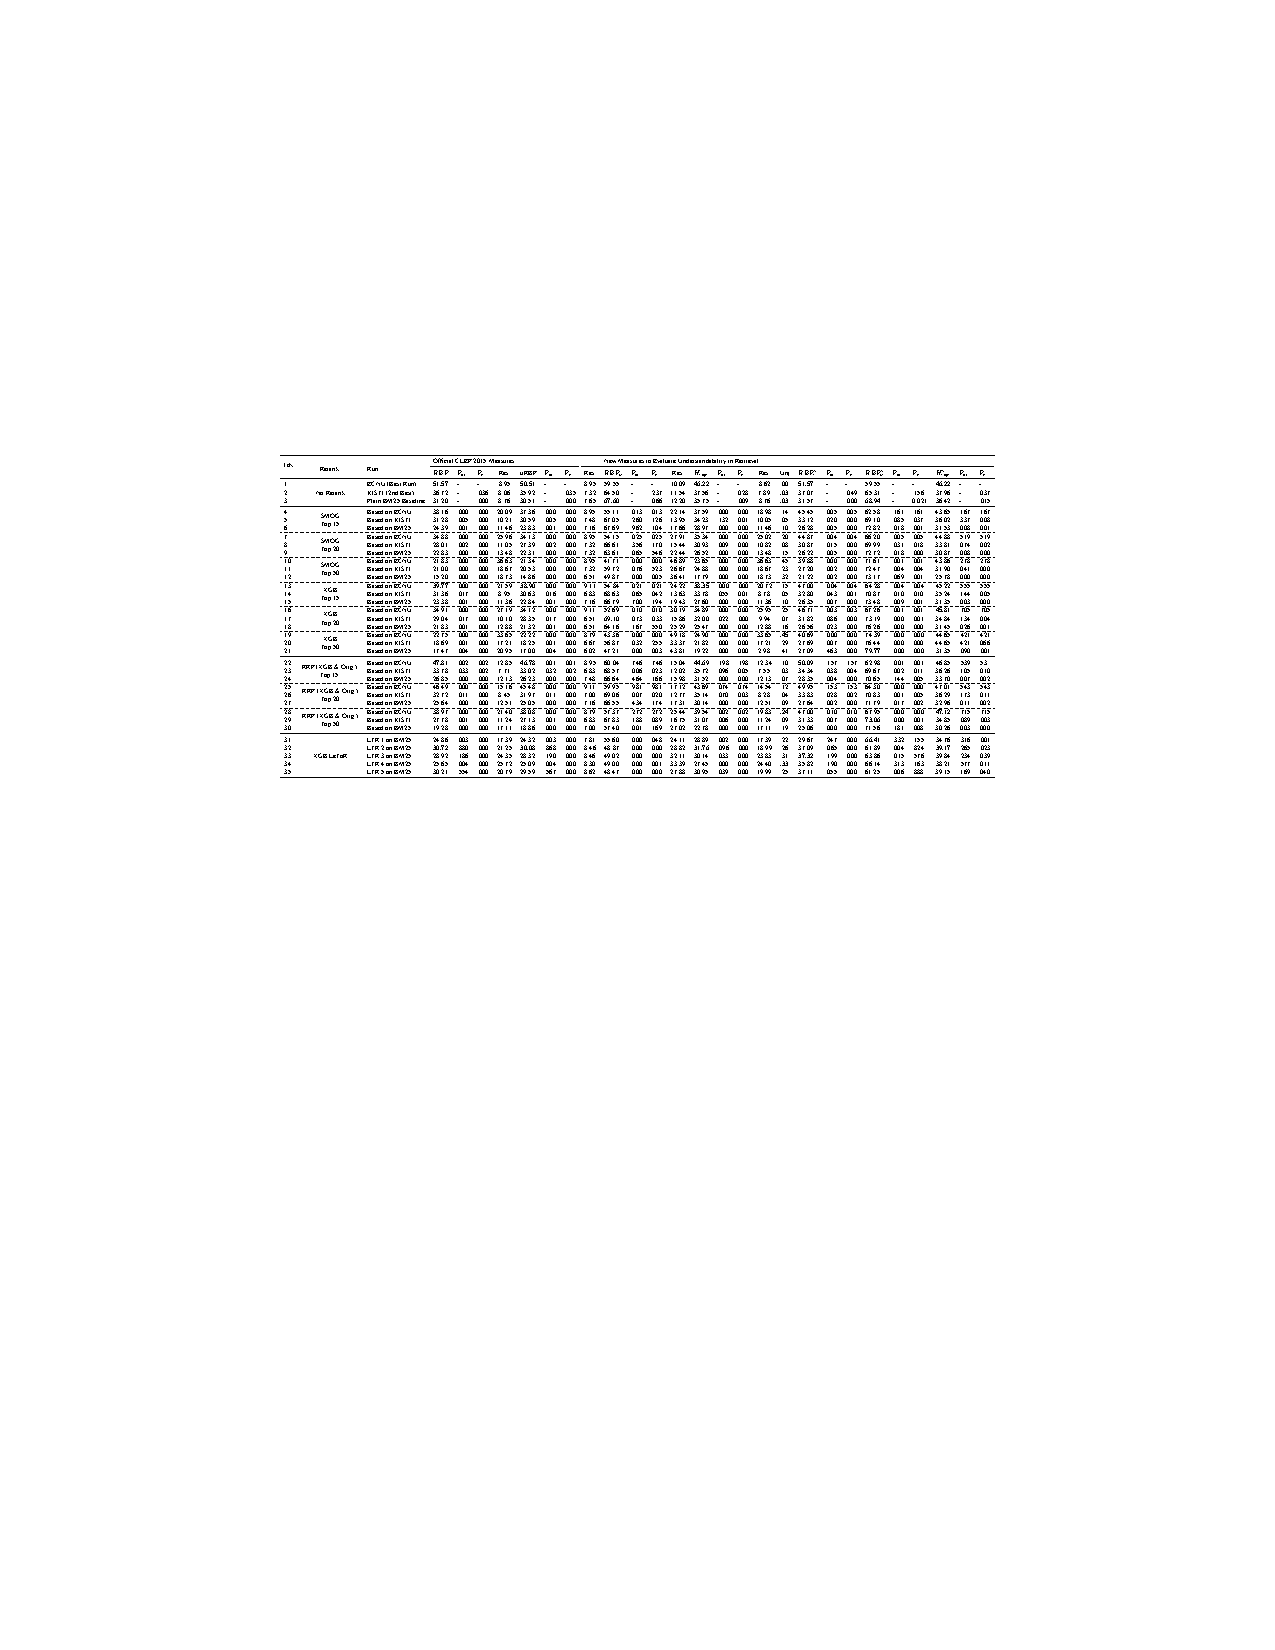
\includegraphics[width=1.0\textwidth]{appendix/results_clef15}
    \caption{Results obtained by integrating understandability estimations within retrieval methods on \textbf{CLEF 2015}. Baseline runs
        are reported at table indices 1-3 (the index column is labelled Index). Re-ranking experiments are reported at indices 4-21. Fusion
        experiments are reported at indices 22-30. Learning to rank experiments are reported at indices 31-35. All measures were
        calculated up to rank n = 10. The highest result of each set of experiments is reported in bold face.}
	\label{fig:dist}
\end{figure}

\newpage
\begin{thebibliography}{1}
	
	\bibitem{palotti15}
	Palotti J, Zuccon G, Hanbury A.
	\newblock The Influence of Pre-processing on the Estimation of Readability of
	Web Documents.
	\newblock In: Proceedings of the 24th ACM International on Conference on
	Information and Knowledge Management. CIKM '15. New York, NY, USA: ACM; 2015.
	p. 1763--1766.
	\newblock \href {http://dx.doi.org/10.1145/2806416.2806613}
	{doi:10.1145/2806416.2806613}.
	
\end{thebibliography}






\end{document}
